\documentclass[9pt]{extarticle}
\usepackage[letterpaper,margin=0.34in]{geometry}
\usepackage[T1]{fontenc}
\usepackage{charter}
\usepackage{euler}
\usepackage{amsmath,amssymb,amsfonts}
\usepackage{microtype}
\usepackage{graphicx}
\usepackage{array,tabularx}
\usepackage{ragged2e}
\pagestyle{empty}
\setlength{\parindent}{0pt}
\setlength{\parskip}{0pt}
\setlength{\jot}{1.5pt}
\setlength{\tabcolsep}{2pt}
\newcommand{\pa}{\partial_{\alpha}}
\newcommand{\QQ}{\mathbb Q}
\newcommand{\DoubleRule}{\par\vspace{3pt}\hrule height 0.65pt\vspace{1.3pt}\hrule height 0.28pt\vspace{5.2pt}}
\newcolumntype{H}{>{\bfseries\raggedright\arraybackslash}p{1.02in}}
\newcolumntype{Y}{>{\raggedright\arraybackslash}X}
\begin{document}
\enlargethispage{24pt}
\vspace*{-10pt}

\noindent
\begin{minipage}[t]{0.63\textwidth}
{\fontsize{12.1}{13.6}\selectfont\bfseries Circle Triangle Square Periods certificate\par}
\end{minipage}\hfill
\begin{minipage}[t]{0.34\textwidth}
\raggedleft{\fontsize{8.4}{9.8}\selectfont Bradley Klee, Mech.An.ika Sol (Open AI)\par}
\end{minipage}
\par\vspace{3.5pt}
\noindent\rule{\textwidth}{0.45pt}
\vspace{7.0pt}

\noindent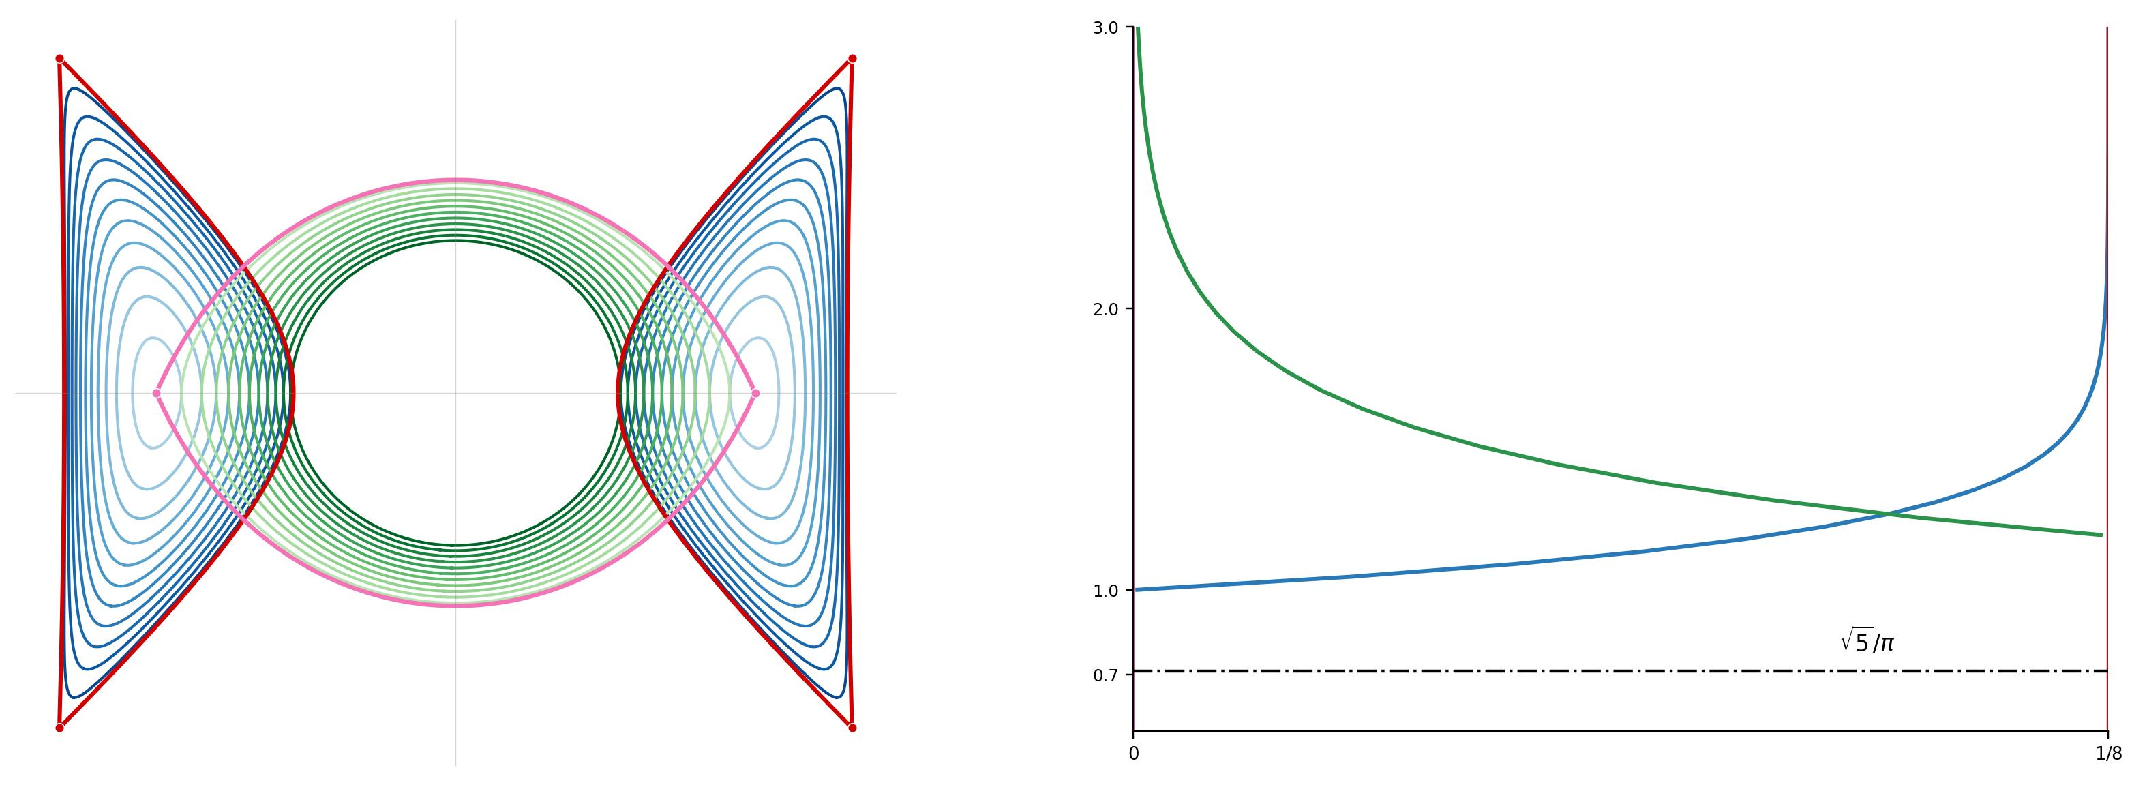
\includegraphics[width=0.985\textwidth]{assets/geometry_period.pdf}
\vspace{-3pt}
\begin{tabularx}{\textwidth}{@{}Y@{\hspace{1.2em}}Y@{}}
\centering\textbf{(a)} Toric section of the curve family $H(p,q)$. &
\centering\textbf{(b)} Periods and Abel's identity. \\
\end{tabularx}
\DoubleRule

{\fontsize{8.95}{11.0}\selectfont
\renewcommand{\arraystretch}{1.30}
\begin{tabularx}{\textwidth}{@{}H@{\hspace{0.10in}}Y@{}}
Curve &
$\displaystyle \alpha=2H(p,q)=p^2+q^2+q^3-3p^2q+\frac{p^4-6p^2q^2+q^4}{4},
\qquad \rho=(2H)_p=p(p^2+2-6q-3q^2).$ \\[7pt]
Period form &
$\displaystyle \omega=\frac{2\,dq}{\rho}=\frac{dq}{H_p}.$ \\[4pt]
Real period &
$\displaystyle T_1(z)=\frac{1}{2\pi}\oint_{\gamma_z^{(1)}}\omega,\qquad
T_1(0)=1,\qquad \gamma_z^{(1)}\subset(p,q)\text{ around }(0,0).$ \\[4pt]
Complex period &
$\displaystyle T_2(z)=\frac{\sqrt5}{4\pi}\oint_{\gamma_z^{(2)}} i\,\omega,\qquad
T_2(1/4)=1,\qquad \gamma_z^{(2)}\subset(ip,q)\text{ around }(0,-1).$
\\[6pt]
Abel's identity &
$\displaystyle
\frac{z(z+6)(4z-1)(8z-1)}{17z-3}
\bigl(T_1(z)T_2'(z)-T_2(z)T_1'(z)\bigr)
=\frac{\sqrt5}{\pi}.$ \\[7pt]
Annihilator &
$\displaystyle A_\alpha=P_0+P_1\pa+P_2\pa^2.$ \\[2pt]
& \hspace{1.25em}$\displaystyle P_0=27-261\alpha+645\alpha^2+408\alpha^3.$ \\[1pt]
& \hspace{1.25em}$\displaystyle P_1=-18+426\alpha-2827\alpha^2+5736\alpha^3+1632\alpha^4.$ \\[1pt]
& \hspace{1.25em}$\displaystyle P_2=\alpha(\alpha+6)(4\alpha-1)(8\alpha-1)(17\alpha-3).$ \\[7pt]
Factorization &
$\displaystyle P_1=P_2'-\frac{34}{17\alpha-3}P_2,$
\qquad
$\displaystyle A_\alpha=(17\alpha-3)^2\pa\!\left(\frac{P_2}{(17\alpha-3)^2}\pa\right)+P_0.$ \\[8pt]
Certificate &
$\displaystyle \Xi=\frac{V(\alpha,p,q)}{\rho^3},\qquad
A_\alpha\circ\omega=d\Xi,$
\qquad
$\displaystyle V=\sum_{j=0}^{9}u_j(\alpha)q^j+p^2\sum_{j=0}^{7}v_j(\alpha)q^j.$
\end{tabularx}
}

\DoubleRule

{\fontsize{8.00}{12.25}\selectfont
\renewcommand{\arraystretch}{1.22}
\begin{tabularx}{\textwidth}{@{}r@{\;}Y@{\hspace{1.5em}}r@{\;}Y@{}}
\multicolumn{2}{@{}l}{\bfseries Numerator: $q^j$ coefficients} &
\multicolumn{2}{l@{}}{\bfseries Numerator: $p^2q^j$ coefficients} \\[1pt]
$u_0={}$ & $-6\alpha(136\alpha^3+411\alpha^2-211\alpha+14)$ &
$v_0={}$ & $-816\alpha^4-650\alpha^3+3475\alpha^2-1089\alpha+102$ \\
$u_1={}$ & $-2(1224\alpha^4-6765\alpha^3+3412\alpha^2-381\alpha+18)$ &
$v_1={}$ & $-3(272\alpha^4-2322\alpha^3+8515\alpha^2-2733\alpha+258)$ \\
$u_2={}$ & $-2448\alpha^4+4410\alpha^3+6337\alpha^2-2811\alpha+210$ &
$v_2={}$ & $-2(816\alpha^3-16195\alpha^2+5646\alpha-543)$ \\
$u_3={}$ & $-816\alpha^4-31170\alpha^3+7331\alpha^2+1719\alpha-66$ &
$v_3={}$ & $-2(11152\alpha^3-37113\alpha^2+11910\alpha-1125)$ \\
$u_4={}$ & $-2(12240\alpha^3+9535\alpha^2-5142\alpha+363)$ &
$v_4={}$ & $-10(1632\alpha^3+6286\alpha^2-2343\alpha+228)$ \\
$u_5={}$ & $-2(2448\alpha^3-6185\alpha^2+2256\alpha+39)$ &
$v_5={}$ & $-2(1632\alpha^3+61502\alpha^2-21579\alpha+2076)$ \\
$u_6={}$ & $14(3842\alpha^2-1473\alpha+60)$ &
$v_6={}$ & $-28(1972\alpha^2-687\alpha+66)$ \\
$u_7={}$ & $2(20162\alpha^2-7665\alpha+348)$ &
$v_7={}$ & $-4(1972\alpha^2-687\alpha+66)$ \\
$u_8={}$ & $36(340\alpha^2-129\alpha+6)$ & & \\
$u_9={}$ & $4(340\alpha^2-129\alpha+6)$ & &
\end{tabularx}
}

\DoubleRule

{\fontsize{8.75}{11.55}\selectfont
\renewcommand{\arraystretch}{1.30}
\begin{tabularx}{\textwidth}{@{}H@{\hspace{0.10in}}Y@{}}
Series &
$\displaystyle T_1(8x)=1+12x+372x^2+15120x^3+706020x^4+35692272x^5+\cdots,$ \\
& $\displaystyle T_2(1/4-100x)=1+108x+24420x^2+6819120x^3+2096600100x^4+681263917488x^5+\cdots.$
\end{tabularx}
}

\end{document}
